
\chapter{확률밀도함수}
\label{density}
\index{PDF}
\index{확률밀도함수 (probability density function)}
\index{지수분포 (exponential distribution)}
\index{분포 (distribution)!지수 (exponential)}
\index{정규분포 (normal distribution)}
\index{분포 (distribution)!정규 (normal)}
\index{가우스 분포 (Gaussian distribution)}
\index{분포 (distribution)!가우스 (Gaussian)}
\index{CDF}
\index{미분 (derivative)}


이번 장에서 사용되는 코드는 {\tt density.py}에 있다.
코드를 다운로드하고 작업하는 것에 대한 정보는 ~\ref{code}을 참조한다.

\section{PDF}

CDF 미분을 {\bf 확률밀도함수 (probability density function)}, PDF라고 한다.
예를 들어, 지수분포 PDF는 다음과 같다.

%
\[ \PDF_{expo}(x) = \lambda e^{-\lambda x}   \]
%
정규분포 PDF는 다음과 같다.
%
\[ \PDF_{normal}(x) = \frac{1}{\sigma \sqrt{2 \pi}} 
                 \exp \left[ -\frac{1}{2} 
                 \left( \frac{x - \mu}{\sigma} \right)^2 \right]  \]
%

$x$ 특정한 값에 대한 PDF를 계산하는 것이 대체로 유용하지는 않다. 결과가 확률이 아니기 때문이다; 확률 {\em 밀도 (density)}다.
\index{밀도 (density)}
\index{질량 (mass)}

물리학에서 밀도는 단위 체적당 질량이다; 질량을 계산하려면, 체적을 곱하거나 혹은 만약 밀도가 상수가 아니라면 체적에 대해 적분해야 한다.

마찬가지로, {\bf 확률 밀도 (probability density)}는 단위 $x$당 확률을 측정한다. 확률 질량을 계산하려면, $x$에 대해서 적분해야 한다. 

{\tt thinkstats2}는 Pdf라는 클래스로 확률밀도함수를 나타낸다.
모든 Pdf 객체는 다음 메쏘드를 제공한다:

\begin{itemize}

\item {\tt Density}, {\tt x}를 인자로 받아 {\tt x}에서 분포 밀도를 반환한다.

\item {\tt Render}는 이산 집합값 대해 밀도를 평가하고 시퀀스 짝을 반환한다: 정렬된 {\tt xs}과 상응하는 확률 밀도{\tt ds}.

\item {\tt MakePmf}, 이산 집합값에 대해 {\tt Density}를 평가하고 Pdf에 그사하는 정규화된 Pmf를 반환한다.
\index{Pmf}

\item {\tt GetLinspace}, {\tt Render}와 {\tt MakePmf}에서 사용되는 기본설정 집합 점(point)을 반환한다.

\end{itemize}  

Pdf는 추상화된 부모 클래스로 의미하는 것은 인스턴스화하면 안된다; 즉, Pdf 객체를 생성할 수 없다. 대신에 Pdf를 상속받아 {\tt Density}과 {\tt GetLinspace} 정의하는 자식 클래스를 정의해야 한다. 
Pdf는 {\tt Render}과 {\tt MakePmf}을 제공한다.

예를 들어, {\tt thinkstats2}는 정규밀도함수를 평가하는 {\tt NormalPdf}라는 이름의 클래스를 제공한다.

\begin{verbatim}
class NormalPdf(Pdf):

    def __init__(self, mu=0, sigma=1, label=''):
        self.mu = mu
        self.sigma = sigma
        self.label = label

    def Density(self, xs):
        return scipy.stats.norm.pdf(xs, self.mu, self.sigma)

    def GetLinspace(self):
        low, high = self.mu-3*self.sigma, self.mu+3*self.sigma
        return np.linspace(low, high, 101)
\end{verbatim}

NormalPdf 객체는 모수 {\tt mu}과 {\tt sigma}을 담고 있다.
{\tt Density}는 {\tt scipy.stats.norm}을 사용하는데 정규분포를 표현한고, 
다른 메쏘드와 더불어 {\tt cdf}와 {\tt pdf}를 제공한다.(~\ref{normal}절 참조).
\index{SciPy}

다음 예제는 BRFSS에 있는 성인여성신장(cm 단위) 평균과 분산으로 NormalPdf를 생성한다(~\ref{brfss}절 참조). 그리고 나서, 평균에서 1 표준편차 지점에 분포 밀도를 계산한다.
\index{표준 편차 (standard deviation)}

\begin{verbatim}
>>> mean, var = 163, 52.8
>>> std = math.sqrt(var)
>>> pdf = thinkstats2.NormalPdf(mean, std)
>>> pdf.Density(mean + std)
0.0333001
\end{verbatim}

결과는 cm 당 확률질량 단위로 약 0.03이다.
한번더, 확률밀도는 그 자체로 의미는 없다. 하지만, Pdf를 플롯으로 그린다면, 분포 형상을 볼 수 있다.

\begin{verbatim}
>>> thinkplot.Pdf(pdf, label='normal')
>>> thinkplot.Show()
\end{verbatim}

{\tt thinkplot.Pdf}은 평활 함수(smooth function)로 Pdf 플롯을 그린다. 
계단함수로 Pmf을 그리는 {\tt thinkplot.Pmf}와 대조된다.
그림~\ref{pdf_example}에 결과가 있다. 다음 절에서 살펴볼 표본에서 추정한 PDF로 함께 플롯되어 그려져 있다.
\index{thinkplot}

Pdf를 근사하는데 {\tt MakePmf}를 사용할 수도 있다.

\begin{verbatim}
>>> pmf = pdf.MakePmf()
\end{verbatim}

기본설정으로, {\tt mu - 3*sigma}에서 {\tt mu + 3*sigma} 사이에 동일 간격을 지닌 101 점이 Pmf에 있다.
선택사양으로 {\tt MakePmf}와 {\tt Render}는 키워드 인자로 {\tt low}, {\tt high}, {\tt n}을 갖는다.

\begin{figure}
% pdf_example.py
\centerline{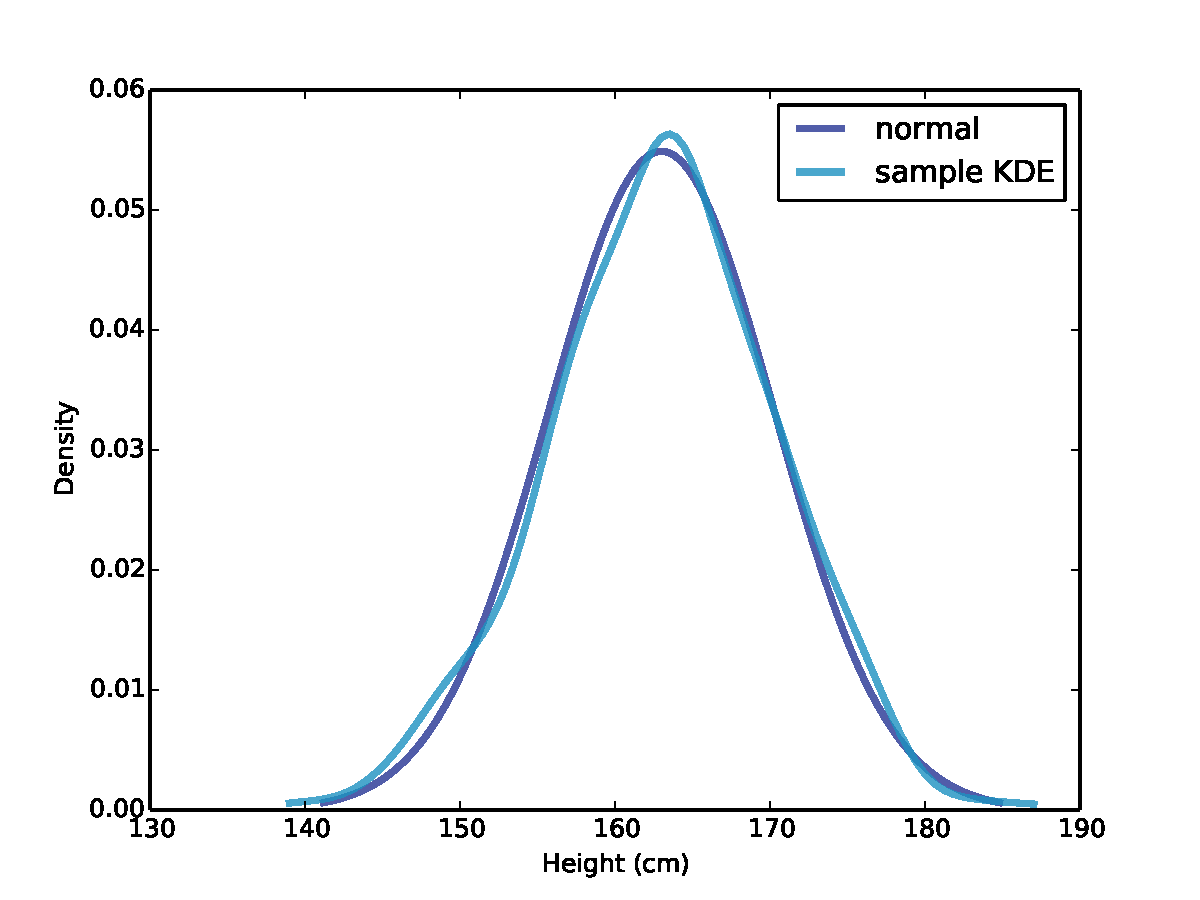
\includegraphics[height=2.2in]{figs/pdf_example.pdf}}
\caption{미국 성인 여성 신장을 모형화하는 정규 PDF, 그리고 $n=500$ 표본으로 핵밀도추정.}
\label{pdf_example}
\end{figure}


\section{핵밀도추정 (Kernel density estimation)} 

{\bf 핵밀도추정 (Kernel density estimation,KDE)}은
표본을 받아 데이터에 적합하는 적절한 평활 PDF를 찾는 알고리즘이다.
\url{http://en.wikipedia.org/wiki/Kernel_density_estimation}  웹사이트에서 좀더 자세한 정보를 얻을 수 있다.

\index{KDE}
\index{핵밀도추정 (kernel density estimation)}

{\tt scipy}에 KDE 구현된 것이 있고, 
{\tt thinkstats2}는 이를 사용해서 {\tt EstimatedPdf}라는 클래스를 제공한다.
\index{사이파이 (SciPy)}
\index{넘파이 (NumPy)}

\begin{verbatim}
class EstimatedPdf(Pdf):

    def __init__(self, sample):
        self.kde = scipy.stats.gaussian_kde(sample)

    def Density(self, xs):
        return self.kde.evaluate(xs)
\end{verbatim}

\verb"__init__"이 표본을 인자로 받아 핵밀도추정값을 계산한다.
결과는 \verb"gaussian_kde" 객체고 {\tt evaluate} 메쏘드를 제공한다.

{\tt Density}가 값 혹은 시퀀스를 인자로 받아 
\verb"gaussian_kde.evaluate"을 호출하고 결과 밀도를 반환한다.
단어 ``가우스 (Gaussian)''가 나오는데 이유는 KDE를 평활하는데 가우스 분포에 기반한 필터를 사용하기 때문이다.
\index{밀도 (density)}

다음에 정규분포에서 표본을 생성하고 표본에 적합하기 위해서 EstimatedPdf를 만드는 예제가 있다.
\index{넘파이 (NumPy)}
\index{EstimatedPdf}

\begin{verbatim}
>>> sample = [random.gauss(mean, std) for i in range(500)]
>>> sample_pdf = thinkstats2.EstimatedPdf(sample)
>>> thinkplot.Pdf(sample_pdf, label='sample KDE')
\end{verbatim}

\verb"sample"은 무작위 신장 500개 리스트다. 
\verb"sample_pdf"는 Pdf 객체로 추정된 KDE 표본정보를 담고 있다.
동일 간격 값의 시퀀스에서 밀도를 평가함으로써 {\tt pmf}는 Pmf 객체로 Pdf를 근사한다.

그림~\ref{pdf_example}에 정규밀도함수와 무작위 신장 500개 표본에 기반한 KDE가 있다. 추정값이 원분포에 좋은 매칭이다.

KDE로 밀도함수를 추정하는 것은 몇가지 목적으로 유용한다. 

\index{thinkplot}
\index{Pmf}

\begin{itemize}

\item {\it 시각화 (Visualization):} 
  프로젝트 탐색단계에서, CDF가 대체로 분포를 가장 잘 시각화한다.
  CDF를 살펴본 후에, 추정 PDF가 분포에 대한 적절한 모형인지 결정할 수 있다.
  만약 그렇다면, CDF에 익숙하지 않은 관계에게 분포를 제시하는데 더 좋은 선택지가 될 수 있다.
\index{시각화 (visualization)}
\index{모형 (model)}

\item {\it 보간 (Interpolation):} 
  추정 PDF는 표본에서 모집단 모형으로 가는 한 방법이다.
  만약 모집단 분포가 매끄럽다고 믿을 이유가 있다면, KDE를 사용해서 표본에 없는 값에 대해 밀도를 보간한다.
\index{보간 (interpolation)}

\item {\it 모의실험 (Simulation):} 
  모의실험은 종종 표본 분포에 기반한다. 
  만약 표본크기가 작다면, KDE를 사용해서 표본분포를 평활하는 것이 적절하다.
  관측점을 중복하기 보다 KDE가 모의실험을 통해서 좀더 가능한 결과값을 탐색하도록 한다.
\index{모의실험 (simulation)}

\end{itemize}


\section{분포 프레임워크 (distribution framework)}
\index{분포 프레임워크 (distribution framework)}

\begin{figure}
\centerline{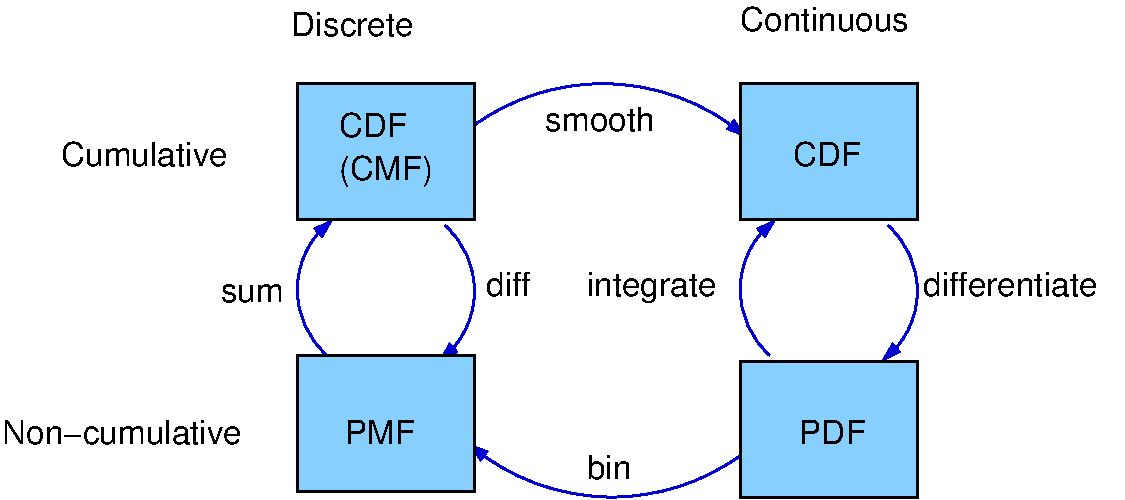
\includegraphics[height=2.2in]{figs/distribution_functions.pdf}}
\caption{분포함수 표현을 연결하는 얼개(framework).}
\label{dist_framework}
\end{figure}

현재까지 PMF, CDF, PDF를 살펴봤다; 잠시 복습 시간을 가져본다.
그림~\ref{dist_framework}에 함수가 어떻게 서로 연관되는지 나타나 있다.
\index{Pmf}
\index{Cdf}
\index{Pdf}

PMF로 시작했는데, PMF는 이산 집합 값에 대한 확률을 나타낸다.
PMF에서 CDF를 얻기 위해서는, 확률 질량을 더해서 누적 확률을 얻는다.
CDF에서 PMF로 돌아가기 위해서는, 누적 확률 차이를 계산한다.
다음 몇 절에 걸쳐 이와 같은 연산을 어떻게 구현했는지 살펴볼 것이다.
\index{누적 확률 (cumulative probability)}

PDF는 연속형 CDF 미분이다; 혹은, 동등하게 CDF는 PDF의 적분이다.
PDF는 값을 확률 밀도로 매핑한다는 것을 기억하라; 확률값을 얻기 위해서,
적분해야 한다.

\index{이산 분포 (discrete distribution)}
\index{연속 분포 (continuous distribution)}
\index{평활 (smoothing)}

이산형에서 연속 분포를 얻기 위해서, 다양한 평활(smoothing) 작업을 수행할 수 있다.
평활의 한 형태는 데이터가 (지수 혹은 정규 분포처럼) 
해석 연속 분포(analytic continuous distribution)에서 왔다고 가정하는 것이다.
또 다른 선택 옵션은 핵밀도추정(kernel density estimation)이다.

\index{지수 분포 (exponential distribution)}
\index{분포 (distribution)!지수 (exponential)}
\index{정규 분포 (normal distribution)}
\index{분포 (distribution)!정규 (normal)}
\index{가우스 분포 (Gaussian distribution)}
\index{분포 (distribution)!가우스 (Gaussian)}

평활의 반대가 {\bf 이산화 (discretizing)}, 혹은 양자화(quantizing)다.
만약 이산 점에서 PDF를 평가한다면, PDF에 근사하는 PMF를 생성할 수 있다.
수치적분(numerical integration)을 사용해서 좀더 잘 근사할 수도 있다.
\index{이산화 (discretize)}
\index{양자화 (quantize)}
\index{구간화 (binning)}

연속CDF와 이산CDF를 구별하기 위해서, 이산CDF는 
``누적 질량 함수 (cumulative mass function)''가 되는 것이 좋을지도 모른다.
하지만, 저자가 알고 있는 바로는, 누구도 그 용어를 사용하지 않는다.
\index{CDF}

\section{Hist 구현}

{\tt thinkstats2}에서 제공되는 기본 기능 사용법을 알아야 한다: Hist, Pmf, Cdf, and Pdf.
다음 절에는 구현된 방식에 대한 상세한 정보가 나와있다.
학습 교재가 좀더 효율적으로 이들 클래스를 사용하는지 도움을 줄 수 있지만,
엄격히 말해서 반듯이 필요하지는 않다.
\index{Hist}

Hist와 Pmf는 \verb"_DictWrapper"라는 부모 클래스를 상속받는다.
클래스 앞 밑줄은 클래스가 ``내부(internal)''라는 것을 나타낸다; 즉,
다른 모듈에 코드로 사용되면 않된다. 명칭이 무엇인지 나타낸다: 
딕셔너리 랩퍼(dictionary wrapper). 
주요 속성은 {\tt d}로, 값을 빈도로 매핑하는 딕셔너리다.

\index{DictWrapper}
\index{내부 클래스 (internal class)}
\index{랩퍼 (wrapper)}

값은 임의 해쉬형(hashable type)이 될 수 있다.
빈도는 정수형이어야 하지만, 임의 숫자형도 될 수 있다.
\index{해쉬 (hashable)}

\verb"_DictWrapper"는 Hist와 Pmf에 대한 적절한 메쏘드를 담고 있는데,
\verb"__init__", {\tt Values}, {\tt Items}, {\tt Render}가 포함된다.
{\tt Set}, {\tt Incr}, {\tt Mult}, {\tt Remove} 변경 메쏘드도 제공한다.
모든 메쏘드는 딕셔너리 연산으로 구현되었다. 예를 들어,
\index{딕셔너리 (dictionary)}

\begin{verbatim}
# class _DictWrapper

    def Incr(self, x, term=1):
        self.d[x] = self.d.get(x, 0) + term

    def Mult(self, x, factor):
        self.d[x] = self.d.get(x, 0) * factor

    def Remove(self, x):
        del self.d[x]
\end{verbatim}

Hist는 또한 {\tt Freq}을 제공하는데 주어진 값에 대한 빈도를 찾는다.
\index{빈도 (frequency)}

Hist 연산자와 메쏘드는 딕셔너리에 기반하고 있어서, 
이들 메쏘드는 상수 시간 연산이다; 즉, Hist가 점점 커짐에 따라 실행시간이 증가하지 않는다.
\index{Hist}


\section{Pmf 구현}
Pmf가 정수 빈도 대신에 값을 부동소수점 확률에 매핑하는 것을 제외하고, 
Pmf와 Hist는 거의 동일하다.
확률을 다 더한 합계가 1 이라면, Pmf는 정규화되었다.
\index{Pmf}

Pmf는 {\tt Normalize} 함수를 제공하는데, 확률을 합을 계산하고 갯수로 나눈다.

\begin{verbatim}
# class Pmf

    def Normalize(self, fraction=1.0):
        total = self.Total()
        if total == 0.0:
            raise ValueError('Total probability is zero.')

        factor = float(fraction) / total
        for x in self.d:
            self.d[x] *= factor

        return total
\end{verbatim}

{\tt fraction}이 정규화한 후에 확률 합계를 알아낸다; 기본 설정값은 1 이다.
만약 전체 확률이 0 이라면, Pmf는 정규화될 수 없어서, {\tt Normalize}는 {\tt ValueError} 오류를 일으킨다.

Hist와 Pmf는 동일한 생성자를 갖고 있다.
인자로 {\tt dict}, Hist, Pmf 혹은 Cdf, 
판다스 시리즈, (값, 빈도) 리스트 쌍, 혹은 값 시퀀스를 받을 수 있다.
\index{Hist}

만약 Pmf를 인스턴스화 한다면, 결과는 정규화된다.
만약 Hist를 인스턴스화 한다면, 결과는 정규화되지 않는다.
정규화되지 않은 Pmf를 생성하기 위해서, 빈 Pmf를  생성해서 변경할 수 있다. Pmf 변경자는 Pmf를 다시 정규화하지 않는다.

\section{Cdf 구현}

CDF가 값을 누적 확률로 매핑해서 Cdf를 \verb"_DictWrapper"로 구현할 수 있다. 하지만 CDF에 있는 값은 정렬되어 있고 \verb"_DictWrapper"에 있는 값은 정렬되어 있지 않다.
또한, 역 CDF를 계산하는 것은 유용하다; 즉, 누적 확률에서 값으로 매핑. 그래서, 저자가 선택한 구현 방법은 두 정렬된 리스트다.
이런 방식으로 이진검색을 사용해서 로그 시간에 앞으로 혹은 역으로 조회할 수 있다.

\index{Cdf}
\index{이진 검색 (binary search)}
\index{누적 확률 (cumulative probability)}
\index{DictWrapper}
\index{역 CDF (inverse CDF)}
\index{CDF, 역 (CDF, inverse)}

Cdf 생성자는 인자로 값 시퀀스 혹은 판다스 시리즈, 값에서 확률로 매핑하는 딕셔너리, (값, 확률) 시퀀스 쌍, Hist, Pmf, 혹은 CDF를 받는다. 혹은 만약 인자가 두개 주어진다면, 두 인자를 각각 정렬된 값 시퀀스와 상응하는 누적확률 시퀀스로 처리한다.

시퀀스, 판다스 시퀀스, 혹은 딕셔너리가 주어지면, 생성자가 Hist를 만든다. 그리고 나서 Hist를 사용해서 속성을 초기화한다.

\begin{verbatim}
        self.xs, freqs = zip(*sorted(dw.Items()))
        self.ps = np.cumsum(freqs, dtype=np.float)
        self.ps /= self.ps[-1]
\end{verbatim}

{\tt xs}는 정렬된 리스트 값이다; {\tt freqs}는 상응하는 빈도 리스트다. {\tt np.cumsum}이 누적 빈도 합계를 계산한다. 
전체 빈도로 나누면 누적확률이 된다.
{\tt n}개 값에 대해서, Cdf를 생성하는 시간은 $n \log n$에 비례한다.
\index{빈도 (frequency)}

다음에 {\tt Prob} 구현한 코드가 있다. 값을 받아 누적 확률을 반환한다.

\begin{verbatim}
# class Cdf
    def Prob(self, x):
        if x < self.xs[0]:
            return 0.0
        index = bisect.bisect(self.xs, x)
        p = self.ps[index - 1]
        return p
\end{verbatim}

{\tt bisect} 모듈은 이진 검색 구현을 제공한다.
그리고, {\tt Value}를 구현했는데 누적 확률을 받아 상응하는 값을 반환한다.

\begin{verbatim}
# class Cdf
    def Value(self, p):
        if p < 0 or p > 1:
            raise ValueError('p must be in range [0, 1]')

        index = bisect.bisect_left(self.ps, p)
        return self.xs[index]
\end{verbatim}

Cdf가 주어지면, 연속 누적 확률 (consecutive cumulative probabilities) 사이 차이를 계산해서 Pmf를 계산할 수 있다.
Cdf 생성자를 호출하고 Pmf를 전달한다면, 
{\tt Cdf.Items}를 호출해서 차이를 계산한다.

\index{Pmf}
\index{Cdf}

\begin{verbatim}
# class Cdf
    def Items(self):
        a = self.ps
        b = np.roll(a, 1)
        b[0] = 0
        return zip(self.xs, a-b)
\end{verbatim}

{\tt np.roll}는 {\tt a} 요소를 오른쪽으로 이동하고,
마지막을 처음으로 ``돌린다(roll)''
{\tt b} 첫 요소를 0으로 바꾸고 나서 {\tt a-b} 차이를 계산한다.
결과는 넘파이 확률 배열이다. 
\index{넘파이 (NumPy)}

Cdf는 {\tt Shift}와 {\tt Scale}를 제공한다. 
Cdf에 값을 변경하지만, 확률은 불변형(immutable)으로 처리되어야 한다.

\section{적률 (Moments)}
\index{적률 (moment)}

어느 때고 표본을 얻고 하나의 숫자로 줄일 수 있다. 그 숫자가 통계량(statistic)이다.
지금까지 살펴본 통계량은 평균, 분산, 중위수, 그리고 사분위수다.

{\bf 원적률 (raw moment)}은 일종의 통계량이다. 만약 $x_i$ 표본 값이 있다면,
$k$번째 원적률은 다음과 같다.

%
\[ m'_k = \frac{1}{n} \sum_i x_i^k \]
%
혹은, 파이썬 표기법으로 표현하면, 다음과 같다.

\begin{verbatim}
def RawMoment(xs, k):
    return sum(x**k for x in xs) / len(xs)
\end{verbatim}

$k=1$일 때, 결과는 표본 평균 $\xbar$가 된다.
다른 원적률은 그 자체로 의미가 있지 않다. 하지만, 다른 계산에 사용된다.

{\bf 중심적률(central moments)}이 더 유용하다. 
$k$번째 중심적률은 다음과 같다.
%
\[ m_k = \frac{1}{n} \sum_i (x_i - \xbar)^k \]
%

혹은 파이썬으로 표현하면 다음과 같다.

\begin{verbatim}
def CentralMoment(xs, k):
    mean = RawMoment(xs, 1)
    return sum((x - mean)**k for x in xs) / len(xs)
\end{verbatim}

$k=2$일 때, 결과는 두번째 중심 적률로 분산으로 인지하고 있을 것이다.
분산의 정의가 왜 이러한 통계량이 적률로 불리는지 힌트를 준다.
각 위치 $x_i$에 자를 따라 추를 달고 평균 주위에서 자를 돌리면, 
회전추의 관성 적률은 값의 분산이다. 만약 관성 적률에 익숙하지 않다면,
\url{http://en.wikipedia.org/wiki/Moment_of_inertia} 웹사이트를 참조한다.  
\index{관성 적률(moment of inertia)}

적률에 기반한 통계를 보고할 때, 단위(unit)에 관한 생각이 중요하다.
예를 들어, 값 $x_i$가 cm 이라면, 첫 원적률은 또한 cm이다.
하지만, 두번째 적률은 cm$^2$이고, 세번째 적률은 cm$^3$... 등등이 된다.

이러한 단위 때문에, 적률은 그 자체로 해석하기 어렵다.
두번째 적률에 대해서 분산에 제곱근을 취한 표준편차를 쓰는 것이 이러한 이유다. 
그러면 $x_i$와 단위가 같아진다.
\index{표준 편차 (standard deviation)}


\section{왜도 (Skewness)}
\index{왜도 (skewness)}

{\bf 왜도 (Skewness)}는 분포 형태를 기술하는 속성이다. 
만약 분포가 중심 경향성 주변에서 대칭이라면, 기울어지지 않았다.
만약 값들이 오른쪽으로 좀더 뻗어져 있다면, ``오른쪽으로 기울어져 (right
skewed)'' 있고, 만약 값들이 왼쪽으로 치우쳐 있다면, ``왼쪽으로 기울어져 (left
skewed''있다.

\index{중심 경향성 (central tendency)}

``기울어짐 (skewed)''을 사용하는 것다는 것이 ``편의(biased)''를 함축하지는 않는다.
단지 왜도는 분포 형태만을 기술한다; 표본 추출과정에 편의가 있는지에 관해 
어떤 것도 나타내지 않는다.

\index{편의 (bias)}
\index{표본 왜도 (sample skewness)}

흔히 몇몇 통계량이 분포 왜도를 계량화하는데 사용된다.
주어진 값 시퀀스가 $x_i$가 주어졌을 때, 
{\bf 표본 왜도 (sample skewness)} $g_1$은 다음과 같이 계산된다.

\begin{verbatim}
def StandardizedMoment(xs, k):
    var = CentralMoment(xs, 2)
    std = math.sqrt(var)
    return CentralMoment(xs, k) / std**k

def Skewness(xs):
    return StandardizedMoment(xs, 3)
\end{verbatim}

$g_1$은 제3 표준 적률로 정규화되었다는 것으로 단위가 없다.
\index{표준 적률 (standardized moment)}

음수 왜도는 분포가 왼쪽으로 기울어짐; 양수 왜도는 분포가 오른쪽으로 기울어짐을 
나타낸다. $g_1$의 규모는 왜도 강도를 나타내지만, 그 자체로 해석하기는 쉽지 않다.

실무에서, 표본 왜도를 계산하는 것이 대게 좋은 생각이 되지는 못하다.
만약 어떤 특이점(outlier)이 있다면, $g_1$에 대해서 균형이 맞지 않는 효과를 미친다.
\index{특이점 (outlier)}

분포 비대칭을 평가하는 또 다른 방법은 평균과 중위수 사이 관계를 살펴보는 것이다.
극단값(extreme value)이 중위수보다 평균에 미치는 효과가 더 크다. 그래서 왼쪽으로 기울어진
분포에서 평균은 중위수보다도 더 작다. 오른쪽으로 기울어진 분포에서 평균은 더 크다.

\index{대칭 (symmetric)}
\index{피어슨 중위수 왜도 (Pearson median skewness)}



{\bf 피어슨 중위수 왜도 계수 (Pearson's median skewness coefficient)}는
 표본 평균과 중위수 차이에 기반한 왜도 측도다.
%
\[ g_p = 3 (\xbar - m) / S \]
%
$\xbar$는 표본 평균, $m$은 중위수, $S$는 표준편차다.
혹은 파이썬에서 코드로 작성한 함수는 다음과 같다.
\index{표준편차 (standard deviation)}

\begin{verbatim}
def Median(xs):
    cdf = thinkstats2.Cdf(xs)
    return cdf.Value(0.5)

def PearsonMedianSkewness(xs):
    median = Median(xs)
    mean = RawMoment(xs, 1)
    var = CentralMoment(xs, 2)
    std = math.sqrt(var)
    gp = 3 * (mean - median) / std
    return gp
\end{verbatim}

이 통계량은 {\bf 강건(robust)}해서 의미하는 바는 특이점 때문에 쉽게 휘둘리지 않는다는 것이다.

\index{강건성 (robust)}
\index{특이점 (outlier)}

\begin{figure}
\centerline{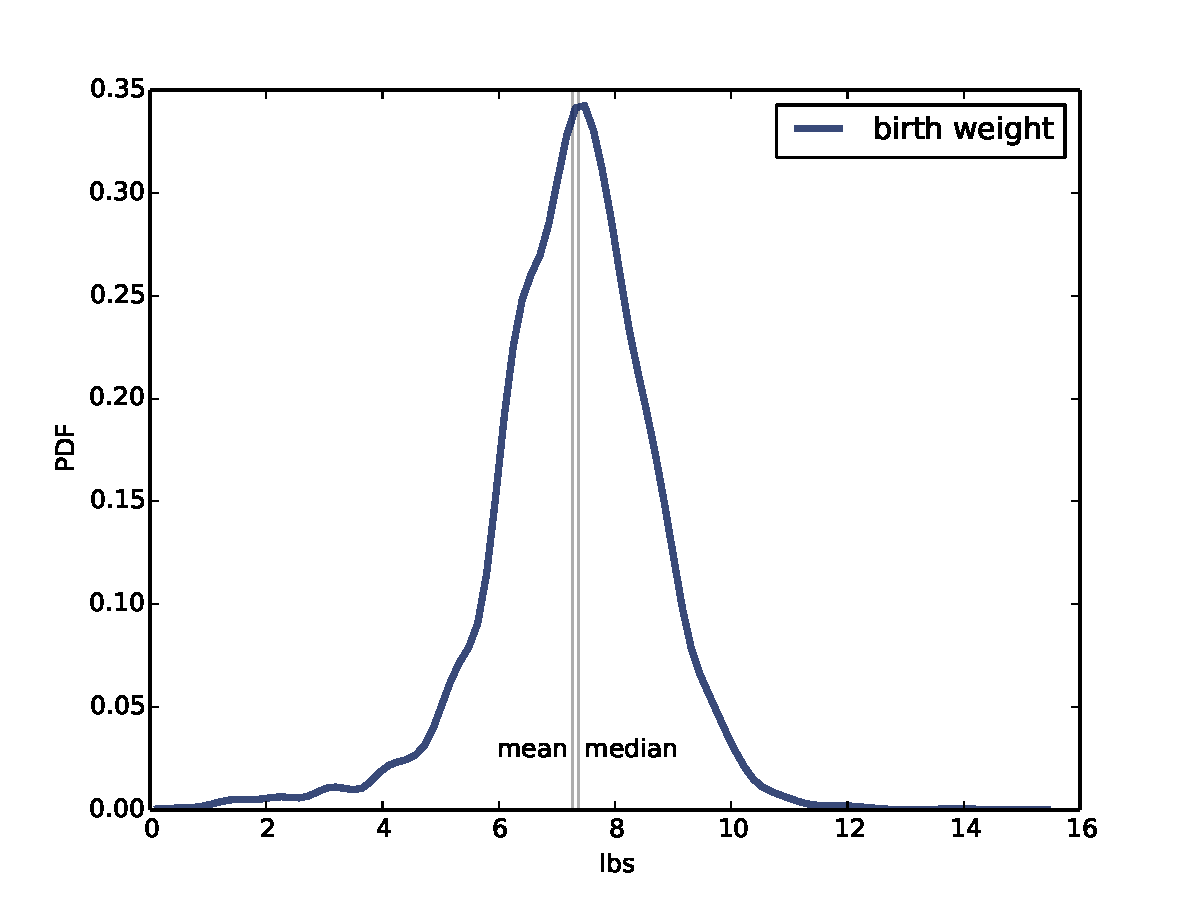
\includegraphics[height=2.2in]{figs/density_totalwgt_kde.pdf}}
\caption{NSFG에서 나온 출생체중 데이터의 추정 PDF.}
\label{density_totalwgt_kde}
\end{figure}

예제로 NSFG 임신 데이터에 있는 출생 체중 왜도를 살펴보자.
다음에 PDF를 추정하고 플롯으로 그리는 코드가 있다.
\index{thinkplot}

\begin{verbatim}
    live, firsts, others = first.MakeFrames()
    data = live.totalwgt_lb.dropna()
    pdf = thinkstats2.EstimatedPdf(data)
    thinkplot.Pdf(pdf, label='birth weight')
\end{verbatim}

그림~\ref{density_totalwgt_kde}에 결과가 있다.
왼쪽 꼬리가 오른쪽 꼬리보다 더 길어 보인다. 
그래서 분포가 왼쪽으로 기울어진 것으로 추측해 볼 수 있다.
평균은 7.27 lbs 으로 중위수 7.38 lbs 보다 다소 작아서 왼쪽으로 기울어진 것과
일관성이 있다. 그리고 두 왜도 계수가 모두 음수다: 표본 왜도는  -0.59; 피어슨 중위수 왜도는 -0.23.
\index{왜도 (skewness)}
\index{dropna}
\index{NaN}

\begin{figure}
\centerline{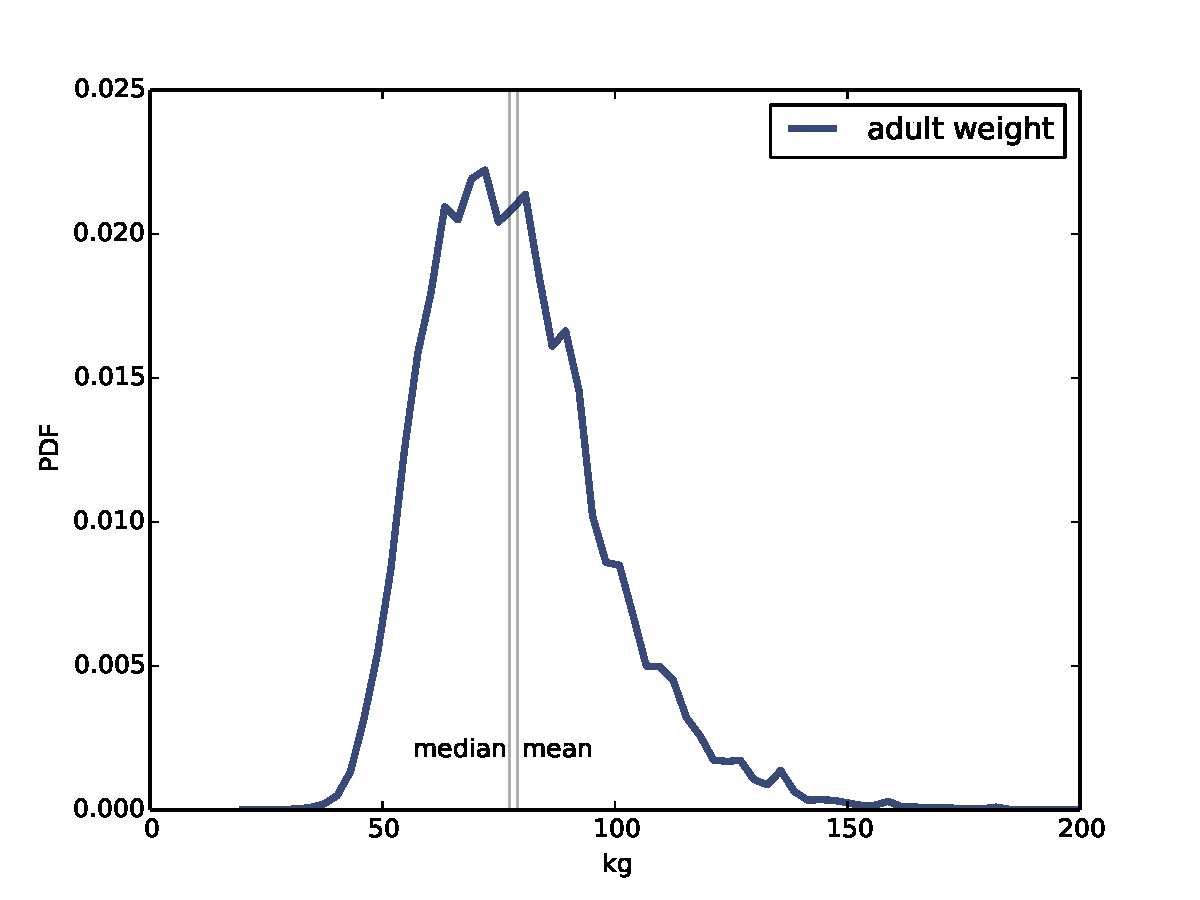
\includegraphics[height=2.2in]{figs/density_wtkg2_kde.pdf}}
\caption{BRFSS에서 나온 성인체중 데이터의 추정 PDF.}
\label{density_wtkg2_kde}
\end{figure}

이제 출생 체중 분포에 대해 BRFSS에 있는 성인 체중 분포와 비교해 보자.
다음에 파이썬 코드가 있다.
\index{thinkplot}

\begin{verbatim}
    df = brfss.ReadBrfss(nrows=None)
    data = df.wtkg2.dropna()
    pdf = thinkstats2.EstimatedPdf(data)
    thinkplot.Pdf(pdf, label='adult weight')
\end{verbatim}

그림~\ref{density_wtkg2_kde}에 결과가 있다.
분포가 오른쪽으로 기울어진 것으로 보인다.
말할 것도 없이, 평균이 79.0으로 중위수 77.3 보다 더 크다.
표본 왜도가 1.1이고 피어슨 중위수 왜도는 0.26이다.
\index{dropna}
\index{NaN}

왜도 계수 부호는 분포가 왼쪽 혹은 오른쪽으로 기울어진 것을 나타내지만,
그것을 제외하고 해석하기는 어렵다.
표본 왜도는 덜 강건하다; 즉, 특이점에 더 좌우된다.
결과로서 덜 믿음이 가는데, 기울어진 분포에 적용될 때, 정확하게 가장 관련될 때 그렇다. 

\index{특이점 (outlier)}
\index{강건성 (robust)}

피어슨 중위수 왜도는 계산된 평균과 분산에 기반한다.
그래서 특이점에 휘둘리기 쉽지만 제3 적률에 의존하지 않기 때문에 좀더 강건하다.
\index{피어스 중위수 왜도 (Pearson median skewness)}


\section{연습문제}

이 연습문제 해답은 \verb"chap06soln.py"에 나와있다.

\begin{exercise}

소득 분포는 유명하게도 우측으로 기울어져 있다.
이번 연습문제에서, 이 치우침이 얼마나 강한지 측정할 것이다.
\index{기울어짐}
\index{소득}

인구동향조사(Current Population Survey, CPS)는 노동통계국(Bureau of Labor Statistics)과 
인구조사국(Census Bureau)의 공동작업으로 소득과 관련된 변수를 연구한다.
2013년에 수집된 데이터는 \url{http://www.census.gov/hhes/www/cpstables/032013/hhinc/toc.htm}에서 다운로드 받을 수 있다.
저자는 가구소득 정보를 갖는 엑셀 파일 {\tt hinc06.xls} 을 다운로드 받아서,
이책의 저장소에서 찾을 수 있는 CSV 파일 {\tt hinc06.csv}로 변환했다.
이 CSV 파일을 불러읽는 {\tt hinc.py} 파일도 함께 있다.

\index{인구동향조사}
\index{노동통계국}
\index{인구조사국}

데이터셋은 소득구간과 해당 구간에 속하는 응답자수의 형태로 되어있다.
가장 낮은 구간은 ``\$5000 이하'' 이하 연간소득을 신고한 응답자가 포함된다.
가장 높은 구간은 ``\$250,000 이상'' 벌어들인 응답자가 포함된다.

이 데이터에서 평균과 다른 통계량을 추정하는데, 하한과 상한에 대해서, 그리고 각 구간에
값들이 어떻게 분포되었는지에 관해 가정을 해야한다.
{\tt hinc2.py} 파일에 {\tt InterpolateSample}이 제공되는데,
데이터를 모형화하는 한 방법을 보여주고 있다.
각 구간에 대한 상한을 담고 있는 {\tt income} 칼럼과 
각 구간에 응답자수를 담고 있는 {\tt freq} 칼럼을 갖는 데이터프레임을 인수로 받는다.
\index{데이터프레임}
\index{모형}

\verb"log_upper"도 인수로 받는데, {\tt log10} 달러로 표현되는 가장 소득이 높은 구간의 상한이다.
기본설정값 \verb"log_upper=6.0" 인데 응답자 가운데에 가장 높은 소득이 $10^6$, 즉 백만불이라는 
가정을 나타낸다.

{\tt InterpolateSample}는 유사표본을 생성한다; 즉,
각 구간에서 실제 데이터와 같은 응답자수를 산출해내는 가구소득 표본이다.
각 구간 소득이 log10 척도로 균등분할됨을 가정한다.

결과로 나온 표본에 대해 중위수, 평균, 기울어짐, 피어슨 기울어짐을 계산하시오.
평균이하 세금을 매길 수 있는 소득이 있는 가구 비율은 얼마인가?
결과가 가정한 상한에 얼마나 의존하는가?

\end{exercise}


\section{용어 사전}

\begin{itemize}

\item 확률밀도함수 (Probability density function, PDF): 
연속 CDF 미분으로 값을 확률 밀도에 매핑하는 함수.
\index{PDF}
\index{확률밀도함수 (probability density function)}

\item 확률밀도 (Probability density): 
  확률을 만들기 위해서 범위 값에 대해 적분할 수 있는 양.
  예를 들어, 만약 값 단위가 cm이라면, 확률밀도는 cm 당 확률 단위가 된다. 
\index{확률 밀도 (probability density)}

\item 핵밀도추정 (Kernel density estimation, KDE): 
  표본에 기반해서 PDF를 추정하는 알고리즘.
\index{핵밀도추정 (kernel density estimation)}
\index{KDE}

\item 이산화 (discretize): 
  연속함수 혹은 이산 함수를 가진 분포를 근사함. 평활(smoothing)의 반대.
\index{이산화 (discretize)}

\item 원적률 (raw moment): 
  거듭 제곱되는 데이터 합계에 기반한 통계량
\index{원적률 (raw moment)}

\item 중심적률 (central moment): 
  평균에서 편차 거듭제곱에 기반한 통계량.
\index{중심적률 (central moment)}

\item 표준적률 (standardized moment): 
  단위가 없는 적률 비율.
\index{표준적률 (standardized moment)}

\item 왜도 (skewness): 
  분포가 얼마나 비대칭인지 나타내는 측도.
\index{왜도 (skewness)}

\item 표본 왜도 (sample skewness): 
  분포 왜도를 정량화하는데 사용되는 적률기반 통계량.
\index{표본 왜도 (sample skewness)}

\item 피어슨 중위수 왜도 계수 (Pearson's median skewness coefficient): 
  중위수, 평균, 표준편차에 기반한 분포 왜도를 정량화하는데 사용되는 통계량.
  \index{피어슨 중위수 왜도 (Pearson median skewness)}

\item 강건성 (robust): 
  특이점에 상대적으로 면역되어 휘둘리지 않는다면 통계량은 강건하다.
\index{강건성 (robust)}

\end{itemize}

